%%%%%%%%%%%%%%%%%%%%%%%%%%%%%%%%%%%%%%%%%
% baposter Portrait Poster
% LaTeX Template
% Version 1.0 (15/5/13)
%
% Created by:
% Brian Amberg (baposter@brian-amberg.de)
%
% This template has been downloaded from:
% http://www.LaTeXTemplates.com
%
% License:
% CC BY-NC-SA 3.0 (http://creativecommons.org/licenses/by-nc-sa/3.0/)
%
%%%%%%%%%%%%%%%%%%%%%%%%%%%%%%%%%%%%%%%%%

%----------------------------------------------------------------------------------------
%	PACKAGES AND OTHER DOCUMENT CONFIGURATIONS
%----------------------------------------------------------------------------------------

\documentclass[a0paper,portrait]{baposter}
\usepackage[utf8]{inputenc}
\usepackage[brazilian]{babel}
\usepackage{verbatim, caption, subfig, array}
\usepackage{cite,url,amsthm,footmisc,bm}
\usepackage{amsmath,graphicx,amssymb,algorithm,algorithmic,graphicx,subfigure,epsfig,multirow,threeparttable,booktabs,bm,mathdots,tabularx}
\usepackage[font=small,labelfont=bf]{caption} % Required for specifying captions to tables and figures
\usepackage{booktabs} % Horizontal rules in tables
\usepackage{relsize} % Used for making text smaller in some places

\graphicspath{{figures/}} % Directory in which figures are stored

\definecolor{bordercol}{RGB}{40,40,40} % Border color of content boxes
\definecolor{headercol1}{RGB}{186,215,230} % Background color for the header in the content boxes (left side)
\definecolor{headercol2}{RGB}{130,130,130} % Background color for the header in the content boxes (right side)
\definecolor{headerfontcol}{RGB}{0,0,0} % Text color for the header text in the content boxes
\definecolor{boxcolor}{RGB}{255,255,255} % Background color for the content in the content boxes

\begin{document}

\background{ % Set the background to an image (background.pdf)
\begin{tikzpicture}[remember picture,overlay]
\draw (current page.north west)+(-2em,2em) node[anchor=north west]
{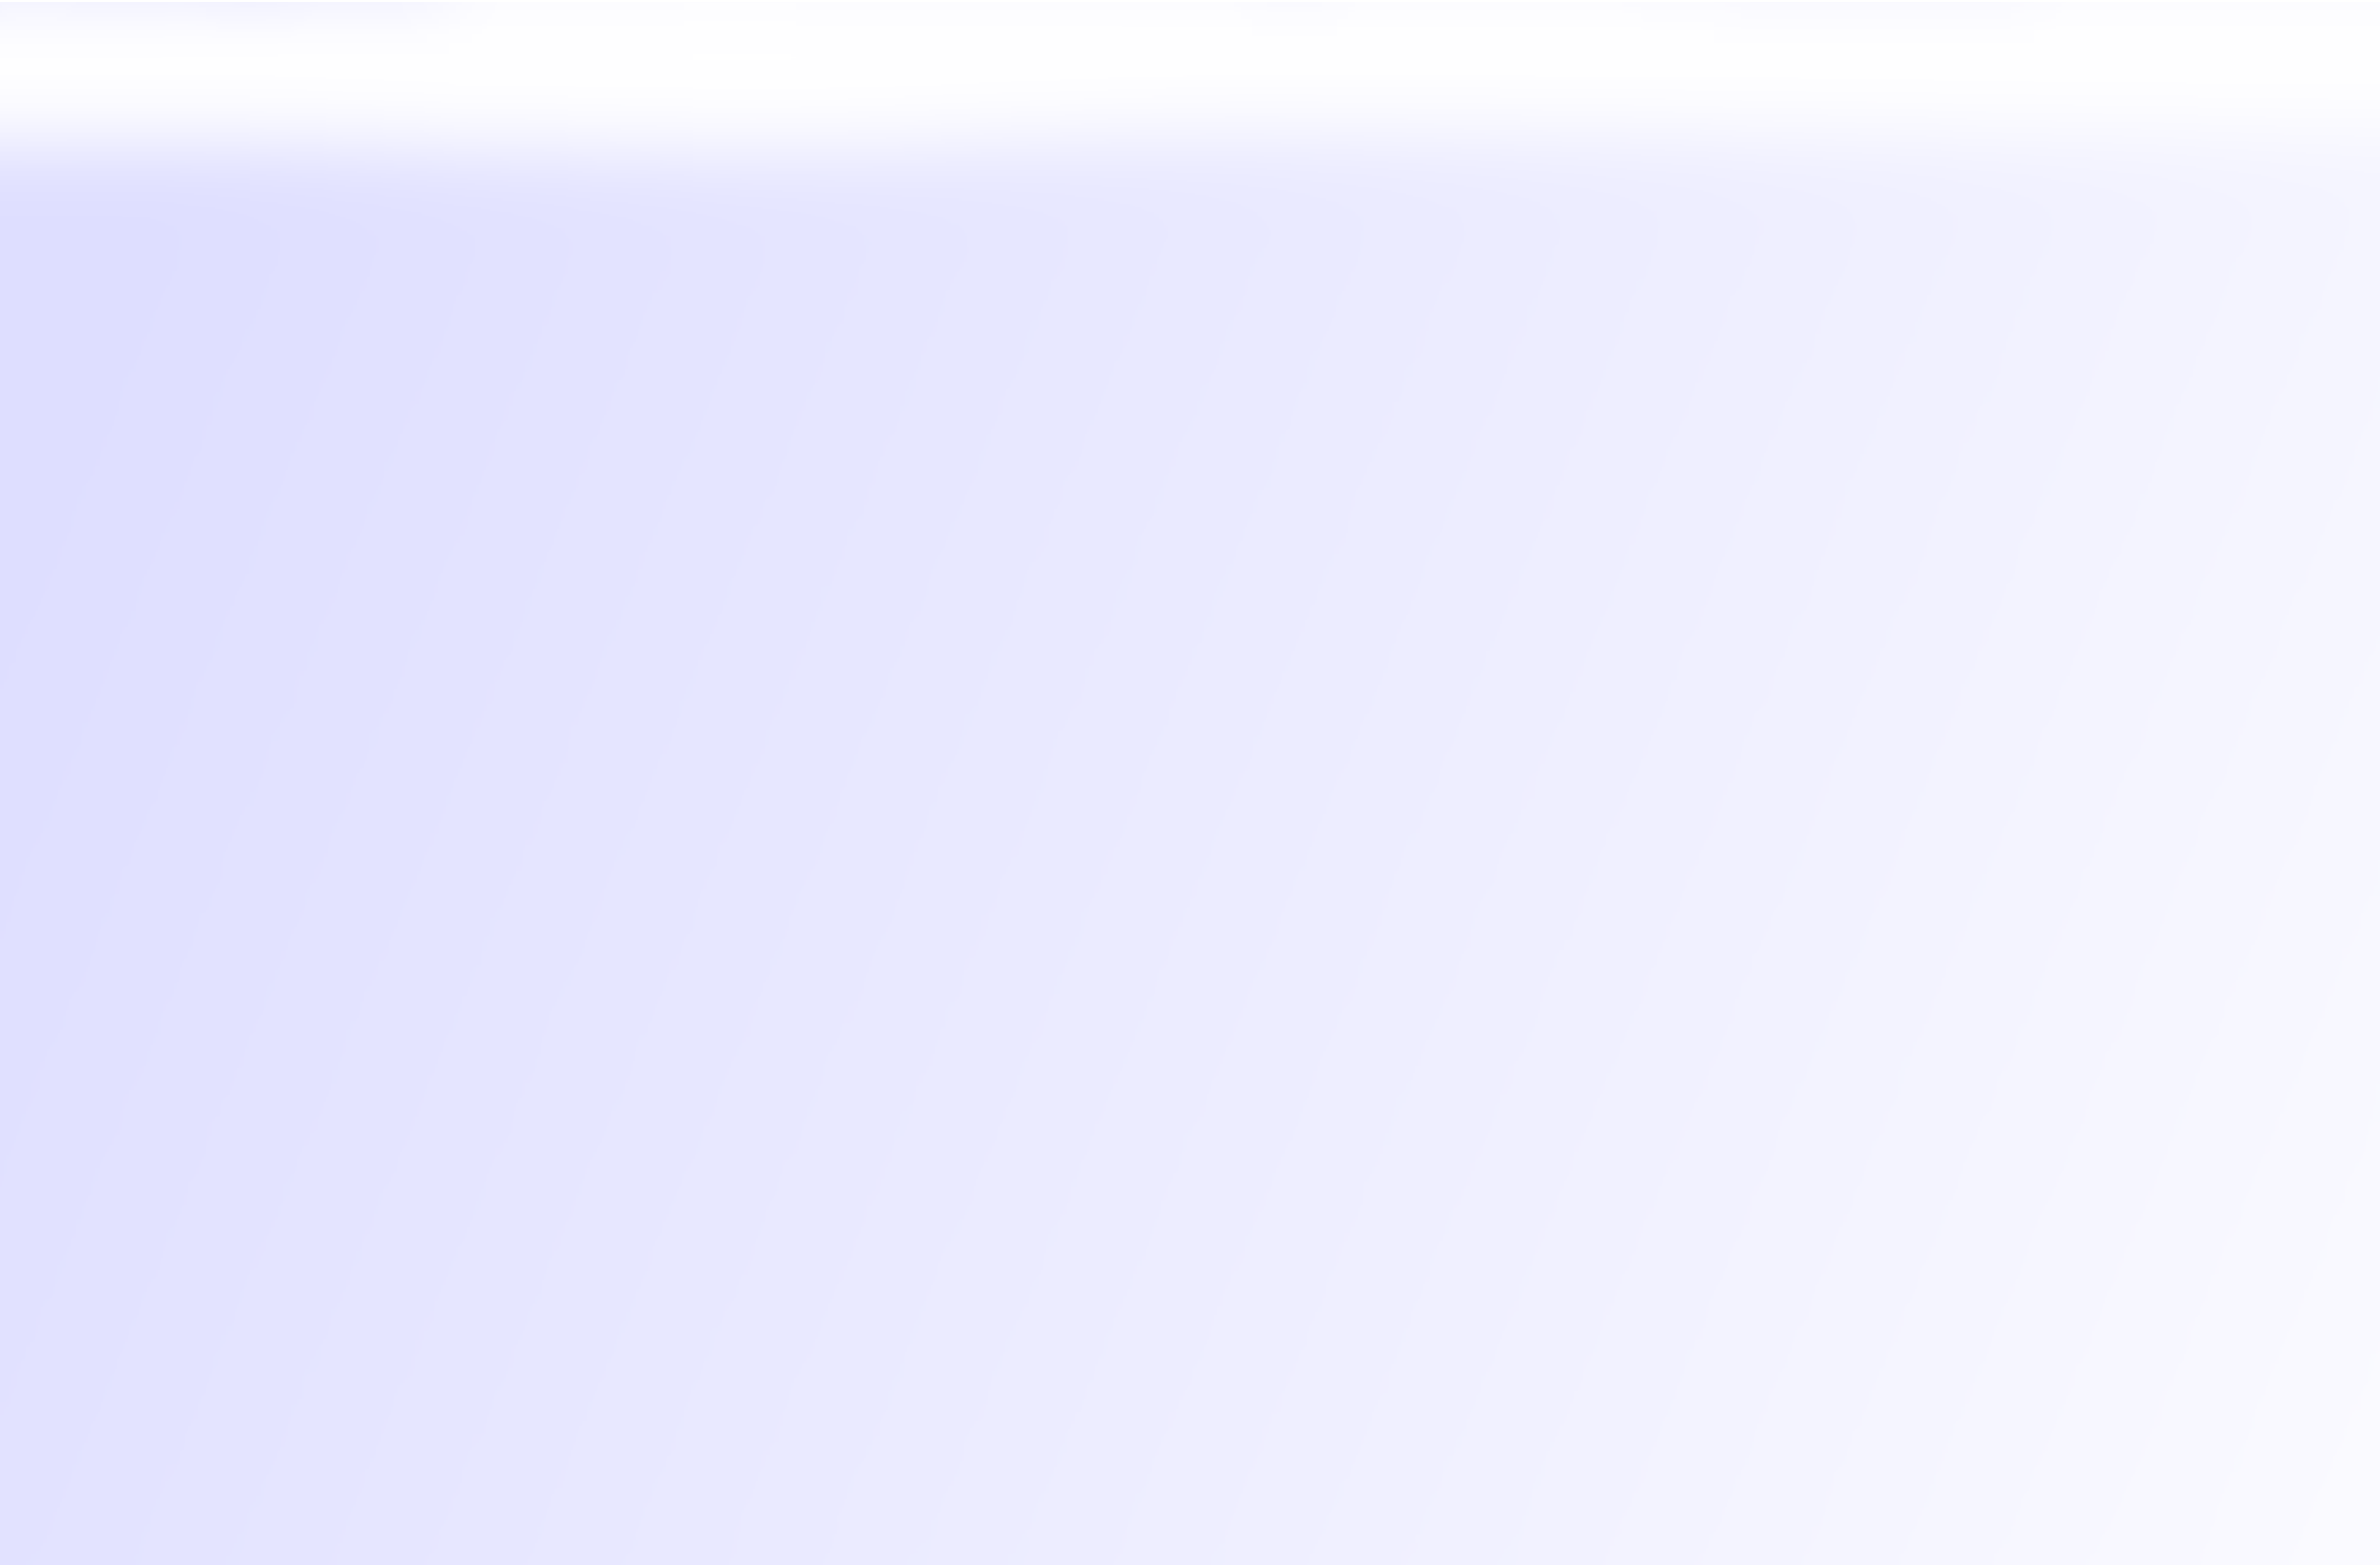
\includegraphics[height=1.1\textheight]{background}};
\end{tikzpicture}
}

\begin{poster}{
grid=false,
borderColor=bordercol, % Border color of content boxes
headerColorOne=headercol2, % Background color for the header in the content boxes (left side)
headerColorTwo=headercol1, % Background color for the header in the content boxes (right side)
headerFontColor=headerfontcol, % Text color for the header text in the content boxes
boxColorOne=boxcolor, % Background color for the content in the content boxes
headershape=roundedright, % Specify the rounded corner in the content box headers
headerfont=\Large\sf\bf, % Font modifiers for the text in the content box headers
textborder=rectangle,
background=user,
headerborder=open, % Change to closed for a line under the content box headers
boxshade=plain
}
{}
%
%----------------------------------------------------------------------------------------
%	TITLE AND AUTHOR NAME
%----------------------------------------------------------------------------------------
%
{\bf \huge \uppercase{Um estudo sobre o quarto elemento fundamental de circuitos: o  \emph{Memristor}}} % Poster title
{\vspace{1em} Cibelly Cristina, Lesly Montúfar e Yasmin Delbany\\ % Author names
{\smaller leslymontufar@ufu.br}} % Author email addresses
{
\includegraphics[width=2.5cm]{logo}} % University/lab logo

%----------------------------------------------------------------------------------------
%	INTRODUCTION
%----------------------------------------------------------------------------------------

\headerbox{Introdução}{name=introduction,column=0,row=0}{

A partir da análise das possíveis combinações entre as quatro variáveis fundamentais de circuitos, Chua [1] 
%\cite{artigo}
 baseando-se no argumento da simetria, postulou que haveria um elemento de circuito faltante, capaz de associar as variáveis carga $q(t)$ e fluxo magnético $\varphi(t)$. Por isso, em 1971, idealizou o novo componente, definido pela relação $d\varphi=M dq$, conforme a Figura \ref{memristor}, e denominou-o \emph{memristor}, uma contração de \emph{memory resistor}. 
 
\vspace{-0.3cm}
\begin{center}
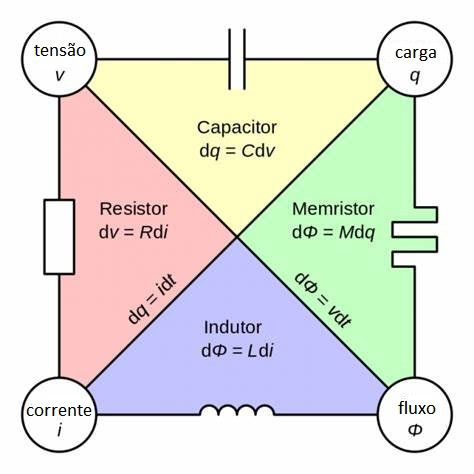
\includegraphics[width=0.8\linewidth]{memristor}
\vspace{-8pt}
\captionof{figure}{Combinações possíveis entre as quatro variáveis fundamentais de circuito.}
\label{memristor}
\end{center}

\vspace{-0.2cm}
%, em português \emph{resistor com memória} 
Considerado, portanto, o quarto elemento fundamental dos circuitos eletrônicos, ao lado do capacitor (1745), resistor (1827) e indutor (1831), o \emph{memristor} destaca-se por apresentar uma propriedade da não-volatilidade, que, aliada a possibilidade de ser trabalhado em escala nanométrica, o torna promissor em aplicações como memórias ReRam e computação neuromórfica.


}

%----------------------------------------------------------------------------------------
%	MATERIALS AND METHODS
%----------------------------------------------------------------------------------------

\headerbox{Modelo de Deriva Linear}{name=methods,column=0,below=introduction}{
O primeiro modelo foi proposto pela \emph{HP Labs}, no qual primeiramente é suposto um campo elétrico uniforme através do dispositivo, que resulta em uma relação linear entre a velocidade de deriva e o campo elétrico líquido. Assim, a memristência $M(q)$ define-se como na Equação (\ref{M:ROFF}), sendo que $Q_D=D^2/\mu_D R_{ON}$ é a carga necessária para mover a deriva de $w(t_0)$, onde $w\rightarrow 0$, para $w(t_D)$, onde $w\rightarrow D$.

\vspace{-0.15cm}
\begin{equation}
M(q)=R_{OFF}\bigg( 1-\dfrac{q(t)}{Q_D}\bigg)
\label{M:ROFF}
\end{equation}

}

%----------------------------------------------------------------------------------------
%	CONCLUSION
%----------------------------------------------------------------------------------------

\headerbox{Conclusão}{name=conclusion,column=0,below=methods}{
Analisa-se os fundamentos físico-químicos e matemáticos do quarto elemento fundamental de circuitos: o \emph{memristor}. Estruturalmente é caracterizado pela redistribuição das nanopartículas dopantes ao longo de sua camada dielétrica, comumente composta por um óxido. No sentido matemático, demonstrou-se que a propriedade da não-volatilidade advém do \emph{pinched hysteresis loop} e que suas características aprimoram-se na redução de escala.

}

%----------------------------------------------------------------------------------------
%	REFERENCES
%----------------------------------------------------------------------------------------

\headerbox{Referências}{name=references,column=0,below=conclusion}{

\smaller % Reduce the font size in this block
\renewcommand{\section}[2]{\vskip 0.05em} % Get rid of the default "References" section title
\nocite{*} % Insert publications even if they are not cited in the poster

\bibliographystyle{unsrt}
\bibliography{sample} % Use sample.bib as the bibliography file
}

%----------------------------------------------------------------------------------------
%	ACKNOWLEDGEMENTS
%----------------------------------------------------------------------------------------



%----------------------------------------------------------------------------------------
%	RESULTS 1
%----------------------------------------------------------------------------------------

\headerbox{Funcionamento estrutural}{name=results1,span=2,column=1,row=0}{ % To reduce this block to 1 column width, remove 'span=2'
%\vspace{-15pt}

\begin{center}
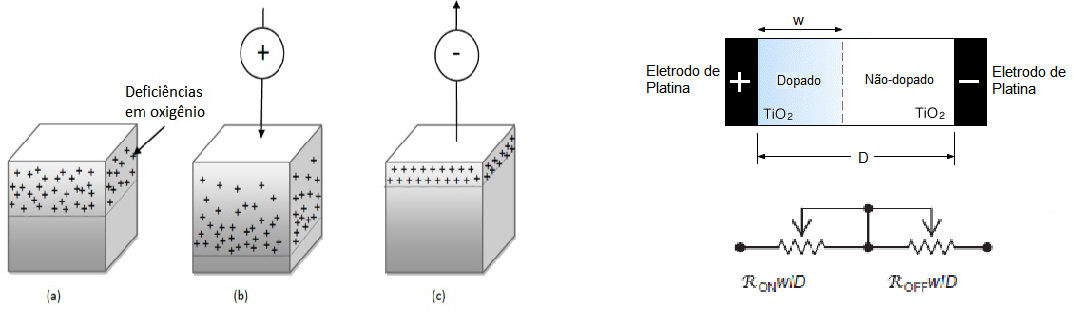
\includegraphics[width=0.95\linewidth]{estrutura2}
\vspace{-8pt}
\captionof{figure}{Mecanismo interno de um \emph{memristor}} \label{ltspice:circuit}
\end{center}


}

%----------------------------------------------------------------------------------------
%	RESULTS 2
%----------------------------------------------------------------------------------------

\headerbox{Fundamentos Matemáticos}{name=results2,span=1,column=1,below=results1,above=bottom}{ % To reduce this block to 1 column width, remove 'span=2'

Um \emph{memristor}, cujo símbolo é apresentado na Figura \ref{simbolo}, modelado a partir das primeiras especificações da \emph{HP Labs} permite extrair as Equações \ref{q}, \ref{q} e \ref{i}.
\begin{center}
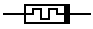
\includegraphics[width=0.75\linewidth]{simbolo}
\vspace{-8pt}
\captionof{figure}{Símbolo de um \emph{memristor}}\label{simbolo} \label{ltspice:circuit}
\end{center}

Considerando um memristor controlado por carga, da parametrização das grandezas carga elétrica $q(t)$, variável de estado $x(t)=w(t)/D$ e corrente elétrica $i(t)$ tem-se:  


\begin{equation}\label{q}
q(t)=Q_D\Bigg(1-\sqrt{1-\dfrac{2}{Q_D\ R_{OFF}}\varphi(t)}\Bigg)
\end{equation} 

\begin{equation}\label{x}
x(t)=1-\sqrt{1-\dfrac{2\, \mu_D}{r\; D^2}\varphi(t)}
\end{equation} 

\begin{equation}\label{i}
i(t)=\dfrac{v(t)}{R_{OFF}\Bigg(\sqrt{1-\dfrac{2\, \mu_D}{r\; D^2}\varphi(t) }\Bigg)}
\end{equation} 
%------------------------------------------------

}

%----------------------------------------------------------------------------------------
---
%	RESULTS 2
%----------------------------------------------------------------------------------------

\headerbox{Análise computacional}{name=results2,span=1,column=2,below=results1,above=bottom}{ % To reduce this block to 1 column width, remove 'span=2'
As Figuras \ref{ltspice:circuit}, \ref{ltspice:tempo} e \ref{ltspice:pinched}, obtidas pelo simulador \emph{LTSPICE}, ilustra o seguinte teorema fundamental: "todo dispositivo de duplo terminal que exibe um \emph{pinched hysteresis loop} no plano tensão-corrente quando conduzido por um sinal DC e/ou senoidal de qualquer frequência é um sistema memristivo".

\vspace{-5pt}
%------------------------------------------------

\begin{center}
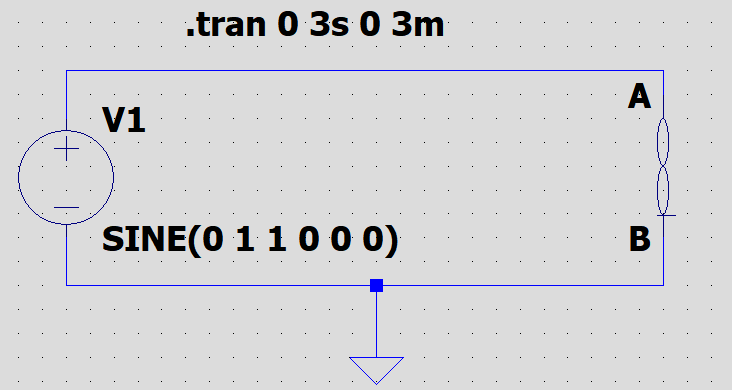
\includegraphics[width=0.8\linewidth]{ltspice001}
\vspace{-8pt}
\captionof{figure}{Circuito \emph{LTSPICE}} \label{ltspice:circuit}
\end{center}

%------------------------------------------------
\vspace{-15pt}
\begin{center}
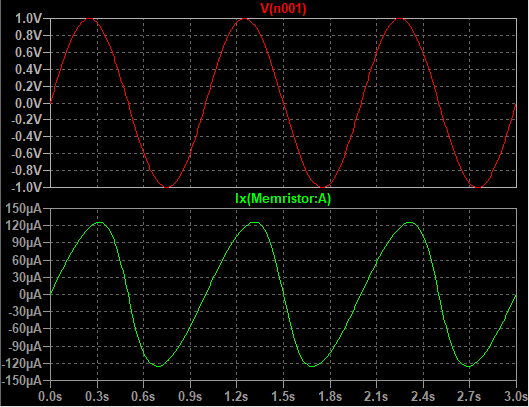
\includegraphics[width=0.8\linewidth]{ltspice002}
\vspace{-8pt}
\captionof{figure}{Tensão e corrente de um \emph{memristor} no domínio do tempo.} \label{ltspice:tempo}
\end{center}

%------------------------------------------------
\vspace{-15pt}
\begin{center}
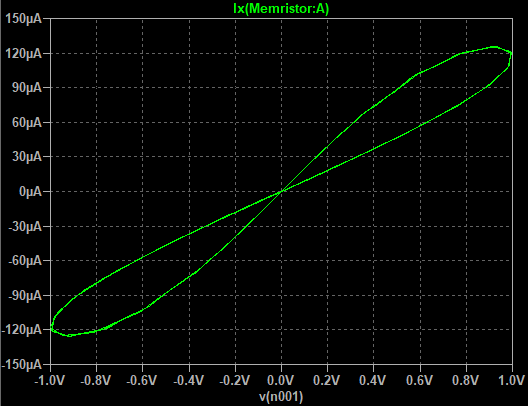
\includegraphics[width=0.8\linewidth]{ltspice003}
\vspace{-8pt}
\captionof{figure}{\emph{Pinched hysteresis loop.}}\label{ltspice:pinched}
\end{center}

%------------------------------------------------
\vspace{-8pt}
 


}

\end{poster}

\end{document}